\chapter{Lo stato attuale}
\thispagestyle{empty}

%Aggiungi un mini indice in questo capitolo se le dimensioni dello stesso iniziano ad essere proibitive.\\
%Parla anche dell'assenza di organi per la misurazione dei consumi (elettrici e termici) e quindi problemi per la valutazione energetica \emph{ante-operam} e per il rispetto ai requisiti \emph{CAM}.\vspace{1em}
Nel primo capitolo si sono descritti in maniera sommaria l'architettura, l'edilizia e gli impianti presenti nell'intero complesso ospedaliero riportando le parole dell'\tit{ing.}{Corrado Beguinot}. In questo capitolo, invece, si vuole dare ampio spazio alle condizioni attuali del suddetto edificio, riportando i dati di input inseriti all'interno dello studio di efficientamento energetico. Prima di iniziare con l'elenco, però, si è voluto descrivere in maniera più dettagliata l'edificio oggetto di questo elaborato di laurea.

Complessivamente tutto il blocco dell'\emph{Edificio 2} ha una superficie calpestabile di \textbf{4200+TOT}\si{m^2}. Per quanto riguarda le porzioni dell'edificio 2 del solo oggetto di questo elaborato di laurea, la superficie calpestabile si attesta a \textbf{TOT}\si{m^2}.

Il suddetto edificio è stato suddiviso per questioni di comodità e calcolo in \emph{5~strutture}:
\begin{itemize}
	\item l'\emph{UTIC} è presente al primo piano dell'edificio alto. Comprende le sale operatorie e le relative degenze.
	\item \emph{Emodinamica} situata al piano terra dell'edificio alto. Comprende la sala operatoria, una sala operatoria minore e le relative sale controllo.
	\item il \emph{Quinto Piano} dell'edificio alto. Qui è presente la \emph{Terapia Intensiva}.
	\item il \emph{Corpo Alto} coincide con l'edificio alto escluse le 3 suddette strutture già menzionate. Sono presenti le degenze, le cucine, i servizi e gli uffici.
	\item il \emph{Corpo Basso} collegato a quello alto tramite un doppio tunnel di cui solo uno è oggetto di studio: sono presenti i laboratori di \emph{Patologia Immunitaria}.
\end{itemize}
Si riporta in Fig.~\vref{planimetriapianoterra} la planimetria del Piano Terra con i contorni colorati che evidenziano le zone di intervento. %Ricorda di dire prima perchè ci sono zone di intervento
\begin{sidewaysfigure}
	\centering
	\caption{Planimetria del Piano Terra dell'Edificio 2. Si notino le due aree di intervento.}
	\label{planimetriapianoterra}
	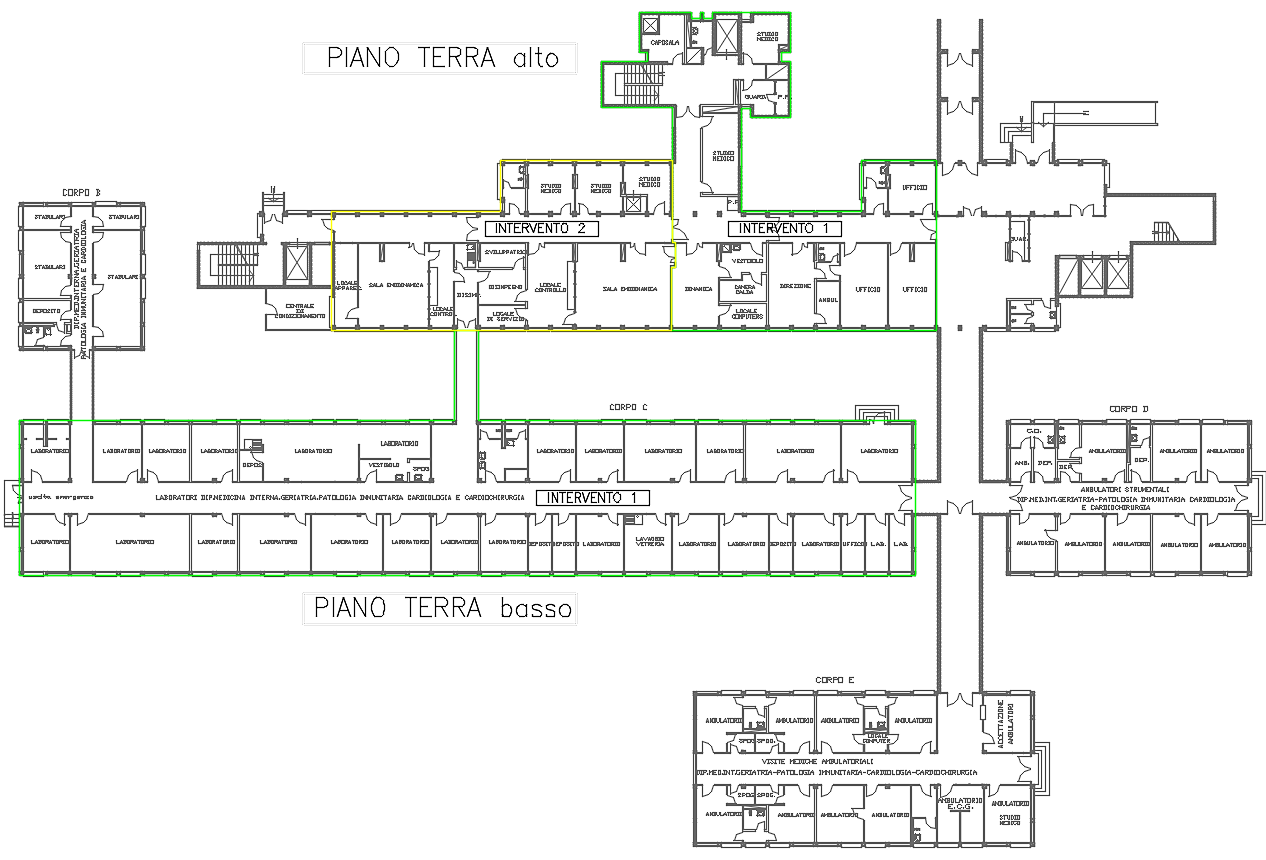
\includegraphics[width=\textheight]{6_2_cap/img/piano_terra}	
\end{sidewaysfigure}

L'edificio 2 preserva tutte le opere edili e impiantistiche realizzate all'epoca della sua costruzione. Non è difficile dedurre, quindi, che allo stato attuale sia le efficienze termiche dell'involucro come quelle termo-meccaniche dell'impianto idro-aeraulico siano quantomeno inferiori a quelle consigliate dalla norma attuale vigente. 

%\begin{itemize}
%	\item componenti opachi
%	\item componenti trasparenti
%	\item ponti termici???
%	\item definizione dei vari locali
%\end{itemize}
%Metti i risultati con tabelle. 
%Inserisci foto in bianco e nero di alcuni componenti finestrati o criticità.
%Prendi in considerazione l'idea di inserire planimetrie da stampare su A3 da piegare all'interno della tesi. 
\section{L'involucro}
\subsection{Componenti opachi}
\subsection{Componenti trasparenti}
\subsection{Definizione locali (norma 10339)}
\section{L'impianto}
\section{I risultati energetici}
\subsection{Stagione Estiva}
Inserisci sia le variazioni dei carichi termici e dell'indice di prestazione energetica.
\subsection{Stagione Invernale}
